\documentclass[a4paper]{article}

\usepackage[english]{babel}
\usepackage[utf8x]{inputenc}
\usepackage{amsmath}
\usepackage{amssymb}
\usepackage{graphicx}
\usepackage[colorinlistoftodos]{todonotes}
\usepackage{fancyhdr}
\usepackage{algorithm}
\usepackage{algpseudocode}
\usepackage{mathtools}


\newtheorem{theorem}{Theorem}[section]
\newtheorem{lemma}[theorem]{Lemma}
\newtheorem{proposition}[theorem]{Proposition}
\newtheorem{corollary}[theorem]{Corollary}

\newenvironment{proof}[1][Proof]{\begin{trivlist}
\item[\hskip \labelsep {\bfseries #1}]}{\end{trivlist}}

\newenvironment{definition}[1][Definition]{\begin{trivlist}
\item[\hskip \labelsep {\bfseries #1}]}{\end{trivlist}}

\newenvironment{example}[1][Example]{\begin{trivlist}
\item[\hskip \labelsep {\bfseries #1}]}{\end{trivlist}}
\newenvironment{remark}[1][Remark]{\begin{trivlist}
\item[\hskip \labelsep {\bfseries #1}]}{\end{trivlist}}

\newcommand{\qed}{\nobreak \ifvmode \relax \else
      \ifdim\lastskip<1.5em \hskip-\lastskip
      \hskip1.5em plus0em minus0.5em \fi \nobreak
      \vrule height0.75em width0.5em depth0.25em\fi}

\pagestyle{fancy}
\setlength{\voffset}{-1in}
\setlength{\textheight}{9.5in}
\setlength{\textwidth}{6.5in}
\setlength{\oddsidemargin}{0in}
\pagenumbering{arabic}
\setlength{\tabcolsep}{1pt}

\title{A Summary of Reliability}

\author{Shangsi Wang}

\date{\today}

\begin{document}
\maketitle

%\begin{abstract}
%We developed a formal theoretical and practical framework to assess reliability from test-restest data which provide guidance for data collection and processing. 
%\end{abstract}

%\section{One paragraph summary}
%In many problems arising in the data science, data collection and processing is the first step toward statistical inference. However, these crucial beginning steps are sometimes done %in an subjective fashion which lacks rigorous guidance and theoretical justification. We propose a definition of reliability as a means to assess the reliability of various data %collection and analysis choices. Moreover, we design a simple and intuitive finite sample estimator of reliability computed from test-restest, which we prove is unbiased and %asymptotically consistent. We showed in theory and through experiments that maximizing reliability minimize a bound on Bayes prediction error. We then apply our reliability approach %to a set of magnetic resonance imaging datasets and find the optimal pre-processing pipeline.



%\section{One page summary}
\noindent In many problems arising in the data science, data collection and processing is the first step toward statistical inference. However, these crucial beginning steps are sometimes done in an arbitrary or subjective fashion which lacks rigorous guidance and theoretical justification. We would like a rigorous theoretical and practical framework to enable investigators to make decisions in collecting and processing heterogeneous datasets, that yield optimal performance on all subsequent inference tasks, including those not yet specified.

\noindent We borrow and extend generalizability theory to apply it to experimental and analysis design. We propose a definition of reliability as a means to assess the reliability of various data collection and analysis choices. Specifically, reliability of a population is defined to be the probability that the distance between two measurements of the same subject is smaller than distance between measurement from an another subject and the measurement from the subject. If we denote $O_{ij}$ the jth measurement of a random subject $i$, then reliability $R$ is defined to be,
\[R \coloneqq P(d(O_{ij},O_{ik})>d(O_{ij},O_{pq})) \]

\noindent Although true population reliability is unknown, we design a simple and intuitive finite sample estimator $\hat{R}$ computed from test-restest dataset. Specifically, $\hat{R}$ is calculated as by counting the triples such that within subject distance and across subject distance and then the count is normalized by a constant $C$, that is
\[\hat{R} \coloneqq \frac{\sum I\{d(O_{ij},O_{ik})>d(O_{ij},O_{pq})\}} {C} \] 
We show that $\hat{R}$ is an unbiased and asymptotically consistent estimator of reliability. Furthermore, we prove that reliability provide a bound on Bayes prediction error for two-class classification problem. Therefore, maximizing reliability in data collection and processing leads to optimal subsequenet prediction performance.


\noindent We conduct a range of numerical experiments demonstrate the utility of our framework in a wide variety of settings. We then apply our reliability framework to a set of magnetic resonance imaging datasets. We are able to comapre datasets and determine which one is the best. Moreover, we can assess reliability of different fMRI pre-processing pipelines and determine which one is optimal. In the figure below, we show the reliability of applying $12$ different processing method on a MRI dataset. We are able to conclude s0g1CC is the best processing method for this dataset.

\begin{center}
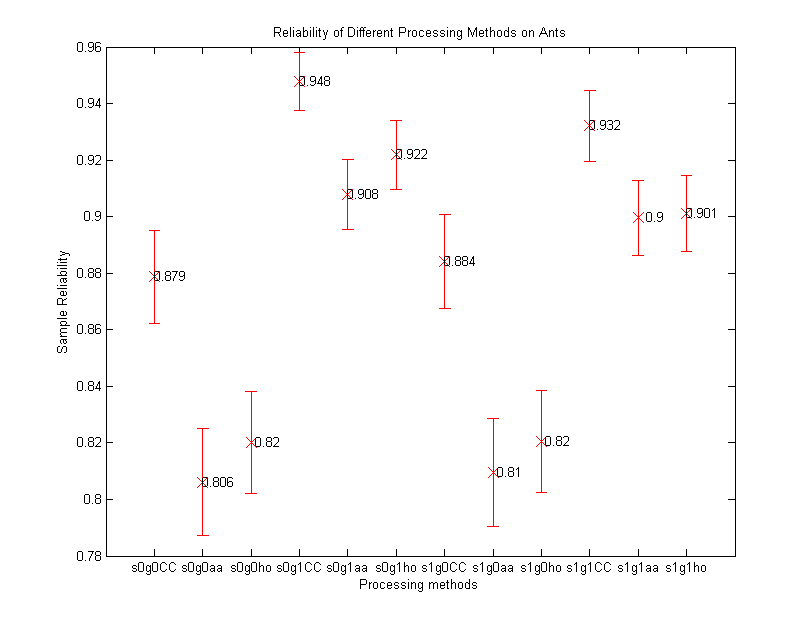
\includegraphics[width=5in,height=3in]{ants_reliability}
\end{center}




\end{document}